\section{OpenFace im Test}
Da mit diesem Verfahren die Landmarks bestimmt werden, aus denen die Gesichtsorientierung abgeleitet wird, sollen die Grenzen dieses Verfahrens ermittelt werden. Von Interesse ist die Bildqualität in der ein Gesicht dargestellt werden muss um dieses noch verarbeiten zu können und wie sehr diese Person von der Kamera abgewandt sein kann.\\
Das Herunterskalieren von Bildern ist nicht das selbe wie eine Aufnahme auf großer Distanz, ist aber ähnlich genug um eine Aussage darüber treffen zu können.\\
Zur Messung wurde der Datensatz von Labeled Faces in the Wild LFW \cite{database_Face} und BIWI Random Forests for Real Time 3D Face Analysis \cite{database_Face_Ori} verwendet.\\
Der LFW Bilddatensatz enthält Abbildungen verschiedener Personen mit einer durchschnittlichen Abbildung der Breite des Kopf von 95 Pixeln. Bei BIWI beträgt die durchschnittliche Breite 78 Pixel und die durchschnittliche Distanz zwischen Kamera und Proband beträgt etwa $95cm$.
\subsection{Auswirkung der Auflösung auf die Detektionsrate}
Durch die Aufgabenstellung muss das Verfahren zuverlässig bezüglich der Distanzen bzw. Darstellungsgröße sein.\\
Bei BIWIk wurde eine Selektion durchgeführt, da die Detektionsrate nur bei $63,4\%$ liegt und durch die Darstellung die Veränderung des Verlauf nur schwer zu erkennen ist.\\
Um die Grenzen der Methode auszuloten wurde das Bild mit unterschiedlichen Faktoren linear skaliert, um so weiter entferntere Gesichter zu simulieren.\\
Um die Detektionsrate zu bestimmen, wurde der Image-Detector von OpenFace auf den skalierten Bildern angewendet und gezählt wie oft der Detektor ein Gesicht erkannt hat. Dabei wurde nicht geprüft ob es sich dabei um ein korrektes Gesicht handelt.\\
Das Ergebnis dieser Messung ist in \autoref{img_lineareverkleinerung} dargestellt. Es ist zu erkennen, dass die Wahrscheinlichkeit einer erfolgreichen Detektion ab einer Skalierung von $0,64$ bei BIWI (Gesicherter mit etwa 50 Pixel Breite) und $0,46$ bei LFW (Gesichter mit 44 Pixel Breite) rapide abnimmt. Bei der in \autoref{Versuch_1} beschriebenen Kamera entspricht dies einer Distanz von etwa $4,5m$.\\
\begin{figure}[p]
	\centering
	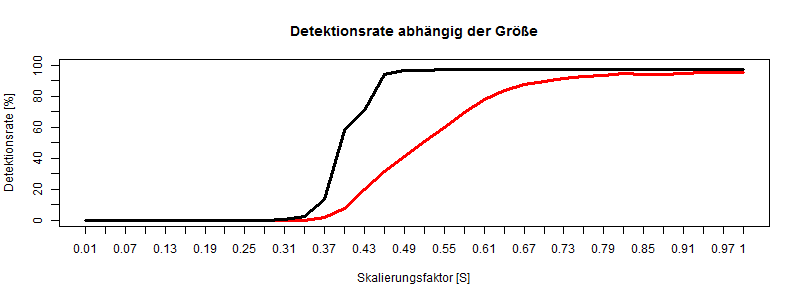
\includegraphics[width=\linewidth]{img_Skalierung/Gesicht_Rate}
	\caption{LFW \cite{database_Face} (schwarz) und BIWI \cite{database_Face_Ori} (grau) um den Skalierungsfaktor verkleinert und gegen die Erkennungsrate aufgetragen}
	\label{img_lineareverkleinerung}
\end{figure}
\subsection{Auswirkung der verschiedenen Skalierungesverfahren auf die Detektion}
\label{OpenFace_skal}
Um die Auswirkung der Skalierungsverfahren zu bestimmen, wurden verschiedene Gesichtsgrößen simuliert, indem alle Bilder von BIWI unf LFW um den angegeben Faktor linear verkleinert wurden und mit den angegebenen Verfahren wieder auf die Originalgröße gebracht.\\
Die Auswirkung der verschiedenen Skalierungsverfahren (Bicubic, Lanczos, Linear, Nearest-Neighbor) auf die Detektionswahrscheinlichkeit ist in \autoref{img_hochskalliern} dargestellt.\\
Es ist zu erkennen, dass die Detektionsrate über einen weiten Bereich, $[1;0,3]$ bei der Skalierung, nur sehr wenig abnimmt. Durch die Vergrößerung können somit jene Gesichter in Skalierungsbereichen ausgewertet werden, die ohne nicht erkennbar sind.\\
Erst bei den sehr kleinen Skalierungen ist ein wirklicher Unterschied zwischen den Verfahren zu erkennen. So nimmt die Detektionsrate bei  Nearest-Neighbor (rot) deutlich früher (BIWI $0,34/27$Pixel und LFW $0,22/21$Pixel) ab, als bei den anderen Verfahren (BIWI $0,22/17$Pixel und $0,13/12$Pixel). Das Bicubic (blau) und Lanczos (grün) Verfahren haben die höchste Detektionsrate und fallen zuletzt ab, wobei Bicubic minimal besser ausfällt.
\begin{figure}
	\centering
	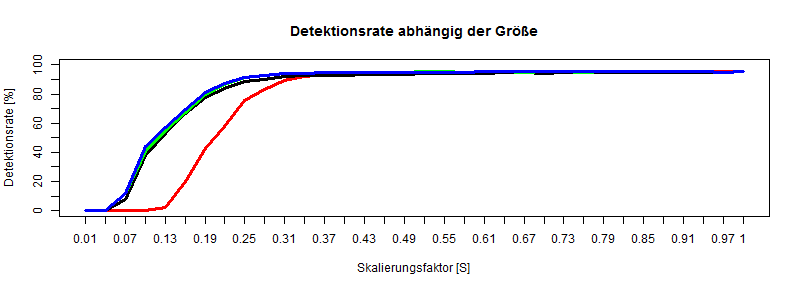
\includegraphics[width=\linewidth]{img_Skalierung/Resize_Rate_Ges}\\
	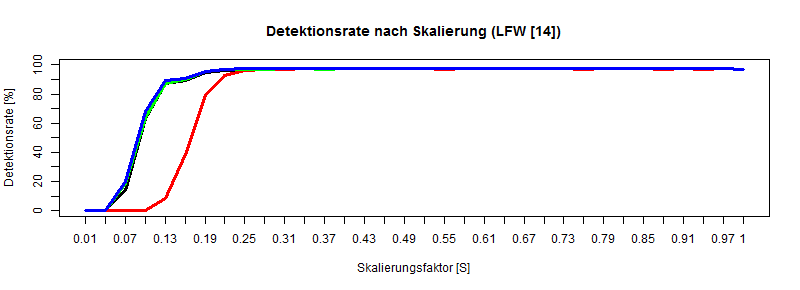
\includegraphics[width=\linewidth]{img_Skalierung/Resize_Rate_lfw}
	\caption{Bilder um den Skalierungsfaktor verkleinert und mit verschiedenen Verfahren wieder vergrößert.\\
		Bicubic (blau), Lanczos (grün), Linear (schwarz), Nearest-Neighbor (rot)}
	\label{img_hochskalliern}
\end{figure}
\subsection{Auswirkung der verschiedenen Skalierungesverfahren auf den Arbeitsbereich bezüglich Rotation}
In \autoref{img_Rot_Dif} ist der Median der Differenz zwischen per OpenFace berechnetem und im Datensatz angegebenem Kopforientierungswinkel aufgetragen.\\
Bei der X-Rotation zeigt sich, dass das Bicubic-Verfahren im Vergleich zu den anderen Verfahren etwa 2 Grad mehr abweicht, ein recht hoher Wert, zumal der Fehler von Lanczos, Linear und Nearest-Neighbor bei etwa $5,8^\circ$ bis zu einer Skalierung von $0,25$ liegt.\\
Der Median der Fehler auf der Y-Achse (nicken) bleibt ebenfalls gering mit $4,2^\circ$ vom Bicubic-Verfahren. Dabei liefern die anderen drei Verfahren nahezu identische Ergebnisse mit etwa $5^\circ$. Die jeweilige Qualität bleibt nahezu konstant bezüglich der Skalierung.\\
Die Z-Rotation wird am besten bestimmt mit einer Abweichung von etwa $2^\circ$ von allen getesteten Verfahren. Dabei ist aber auch zu beachten, das dieser Wertebereich im Datensatz deutlich geringer ausfällt, als bei den anderen beiden Rotationen.\\
Für alle Berechnungen zeigt sich, das der Fehler konstant bleibt, bis zu der Skalierung von $0.25$, bei der auch die Detektionsrate deutlich abfällt.\\
Neben der Qualität der bestimmten Winkel, ist auch der Arbeitsbereich von Interesse in dem Gesichter bei verschiedenen Skalierungen noch erkannt werden können. Ein Gesicht das außerhalb dieses Bereiches liegt kann nicht erkannt und ausgewertet werden.\\
In \autoref{img_Rot_Max} sind die Quantile bei $50\%; 80\%; 99\%$ und der Maximalwert, von den Rotationswinkel der Bilder aus BIWI \cite{database_Face_Ori} dargestellt, in denen ein Gesicht erkannt wurde. Durch den großen Unterschied zwischen dem $80\%$-Wert, $99\%$-Wert und dem Maximalwert liegt die Vermutung nahe, dass es sich bei diesen Werten um falsch detektierte Bilder handelt Dennoch kann eine Rotation des Kopfes von $45\%$ in alle Richtungen erkannt und ausgewertet werden.\\
Eine genaue Darstellung der Messung ist in \autoref{Abbildungen} abgebildet, für die X-Rotation \autoref{img_X_Rot_Skal}, Y-Rotation \autoref{img_Y_Rot_Skal} und Z-Rotation \autoref{img_Z_Rot_Skal}.
\begin{figure}
	\centering
	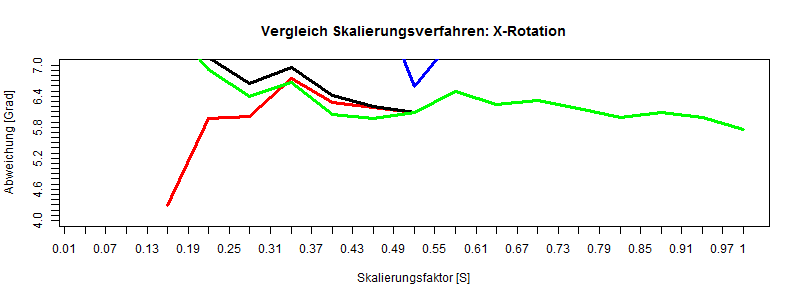
\includegraphics[width=\linewidth]{img_Skalierung/Skal_Diff_RX}
	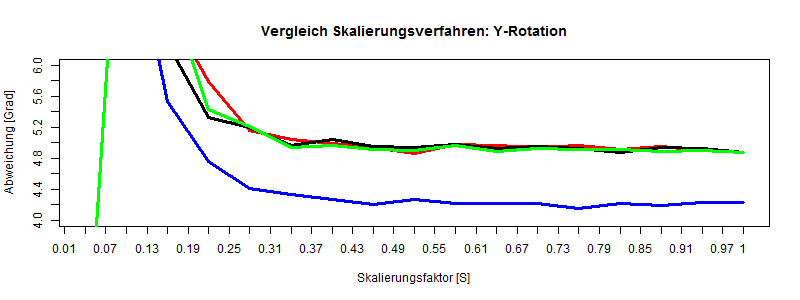
\includegraphics[width=\linewidth]{img_Skalierung/Skal_Diff_RY}
	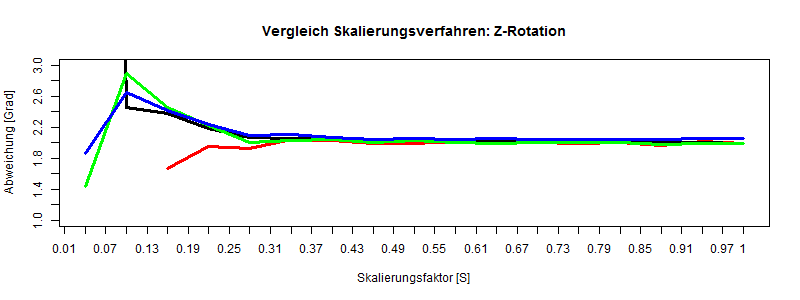
\includegraphics[width=\linewidth]{img_Skalierung/Skal_Diff_RZ}
	\caption{Dargestellt ist der Median der Abweichung zwischen der berechneten Drehung und der des Datensatzes.\\
		Bicubic (blau), Lanczos (grün), Linear (schwarz), Nearest-Neighbor (rot)}
	\label{img_Rot_Dif}
\end{figure}
\subsection{Auswirkung der Skalierungsverfahren auf die Positionsbestimmung}
Für eine zuverlässige Auswertung ist auch die Bestimmung der Position von Interesse. Zur Berechnung der Position auf BIWI wurde eine Brennweite der Kinekt-Kamera auf $531,15$ geschätzt, da es keine Angabe für den Datensatz gab.\\
Der Median der Differenz zwischen Datensatz und Rechnung ist in \autoref{img_Pos_Dif} dargestellt. Bei sehr kleinen Skalierungen existieren durchaus auch sehr große Fehler, diese wurden allerdings bei der Darstellung abgeschnitten, da bei dieser Größe die Detektionsrate so klein ist, dass die Ergebnisse nahezu irrelevant werden.\\
Aus der Abbildung ist zu entnehmen, dass die Position in horizontaler und vertikaler Richtung auf etwa $2,5cm$ genau bestimmt werden kann, die Distanz (Tiefe) auf etwa $2,8cm$ genau. Dies ist selbst bei sehr klein skalierten Bildern möglich.\\
Nearest-Neighbor hat bei der Berechnung der X-Position die geringste Abweichung zu den anderen getesteten Verfahren mit einem unterschied von etwa $1mm$.\\
Bei der Bestimmung der Y-Position hingegen, ist der Unterschied zwischen den vier Verfahren minimal. Die Differenz beträgt weniger als $1mm$ und keines der Verfahren zeugt einen aussagekräftigen Unterschied zu den anderen.\\
Eine ausführliche Darstellung der Messung ist in \autoref{img_X_Pos_Skal}, \autoref{img_Y_Pos_Skal} und \autoref{img_Z_Pos_Skal} dargestellt.
\begin{figure}
	\centering
	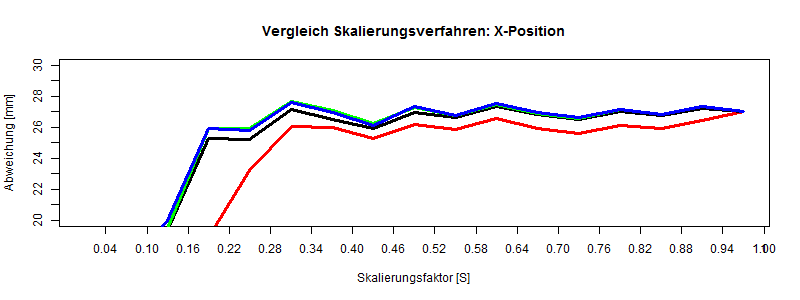
\includegraphics[width=\linewidth]{img_Skalierung/Skal_Diff_TX}
	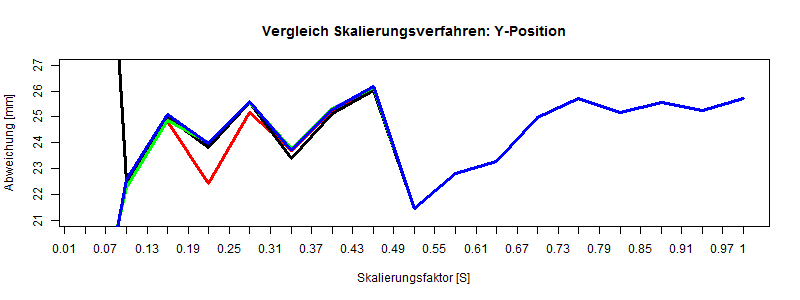
\includegraphics[width=\linewidth]{img_Skalierung/Skal_Diff_TY}
	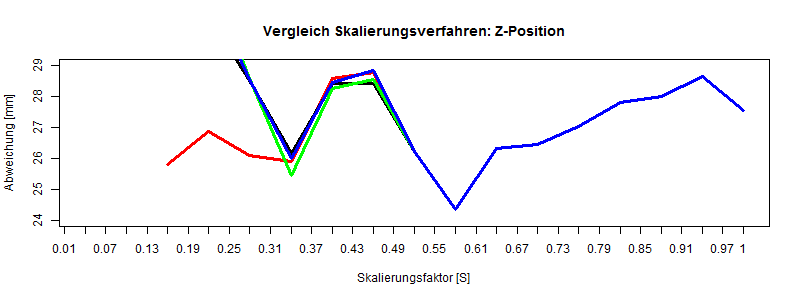
\includegraphics[width=\linewidth]{img_Skalierung/Skal_Diff_TZ}
	\caption{Dargestellt ist der Median der Abweichung zwischen der berechneten Drehung und der des Datensatzes.\\
		Bicubic (blau), Lanczos (grün), Linear (schwarz), Nearest-Neighbor (rot)}
	\label{img_Pos_Dif}
\end{figure}
\subsection{Auswirkung von Pixelrauschen auf die Detektion}
Mit diesem Test soll geprüft werden, welches der Verfahren auch stabil gegenüber Rauschen ist um einen besseren Eindruck für die Verwendbarkeit bei realen Aufnahmen zu erhalten.\\
Das Rauschen wird simuliert, indem für jedes Pixel eine Wahrscheinlichkeit von $50\%$ besteht auf eine gleichverteilte Abweichung von $\pm 10\%$ des originalen Farbwertes. Die Bilder von LFW \cite{database_Face} wurden entsprechend verkleinert, mit Rauschen versehen um sie anschließend mit den unterschiedlichen Verfahren zu vergrößern. Dieser Vorgang wurde für jedes Bild viermal wiederholt um Zufälligkeiten bei der Rauschsimulation zu vermeiden.\\
Wie zu erwarten ist Nearest-Neighbor am schlechtesten, aber auch zwischen den anderen Verfahren sind nun Unterschiede zu erkennen, siehe \autoref{img_hochskalliern_nois}. Die gesamte Erkennungsrate ist deutlich kleiner als ohne Rauschen, wobei der Skalierunfsfaktor von $0.22$, ab welcher die Erkennungsrate rapide abfällt, beibehalten wird.
\begin{figure}
	\centering
	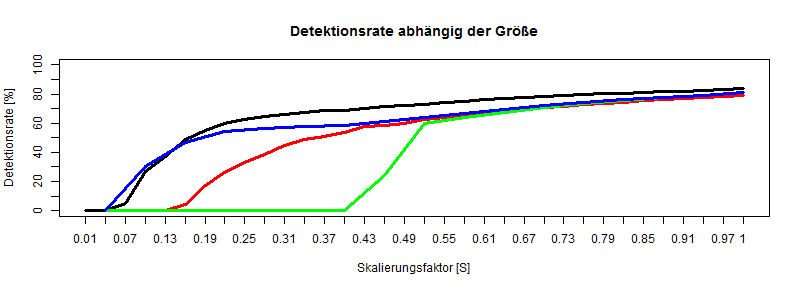
\includegraphics[width=\linewidth]{img_Skalierung/Hochskalliern_Nois}
	\caption{Bilder aus Labeled Faces in the Wild \cite{database_Face}, mit dem X-Faktor verkleinert, um jedes Pixel mit $50\%$ Wahrscheinlichkeit auf $\pm 10\%$ Gleichverteilung der Abweichung\\Bicubic (blau), Lanczos (grün), Linear (schwarz), Nearest-Neighbor (rot)}
	\label{img_hochskalliern_nois}
\end{figure}
\subsection{Auswirkung der verschiedenen Rechenverfahren für die Position}
Um die Qualität der Berechnung auf verschiedenen Distanzen zu ermitteln, wurde der BIWI Datensatz \cite{database_Face_Ori} verwendet, da für jedes Gesicht die Position und Orientierung bekannt ist.
Die durchschnittliche Distanz zwischen Kamera und Kopf beträgt ca $70cm$ bei einer Kopfbreite von 78 Pixel. Um die verschiedenen Distanzen zwischen Probanden und Kamera zu simulieren, wurden die Bilder mit dem angegebene Skalierungsfaktor (X-Achse) linear verkleinert.\\
Da verschiedene Verfahren zur Bestimmung der Position und Orientierung zur Verfügung stehen, sollen diese miteinander verglichen werden. Zur Bestimmung wurde nur das RGB-Bild verwendet und nicht zusätzlich die Tiefenaufnahme, da diese in der Anwendung auch nicht vorhanden ist.
\subsubsection{Position}
Zur Bestimmung der Position gibt es zwei Verfahren, die direkte mittels Brennweite und Skalierung oder Überführungsmatrix von 3D zu 2D Landmarks arbeiten.\\
Die Funktionen PoseCamera und PoseWorld verwenden die einfache Bestimmung mittels Skalierung und CorrectPoseCamera und CorrectPoseWorld die Überführung von 3D und 2D Landmarks, daher überlagern sich die Linien in \autoref{img_Verfahren_Pos}, da die jeweiligen Verfahren nach dem selben Prinzip rechnen.\\
Der schnelle Abfall der Genauigkeit bei der Skalierung $0,25$ ist an der selben Stelle an der auch die Detektionsrate stark absinkt, siehe \autoref{OpenFace_skal}. Somit kann das Verfahren bis zu seiner Grenze eingesetzt werden und erst, wenn die Detektion schwierig wird steigt auch der Fehler.
\begin{figure}
	\centering
	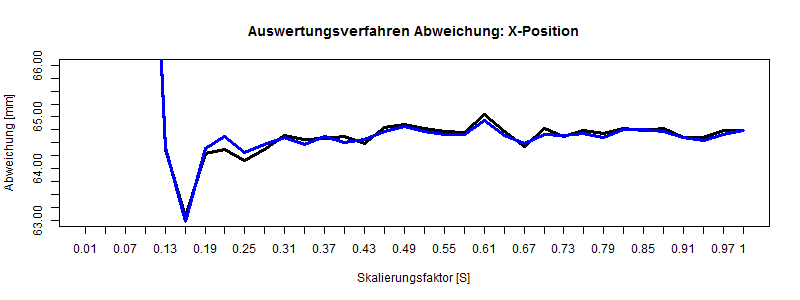
\includegraphics[width=\linewidth]{img_Skalierung/Verfahren_TX}
	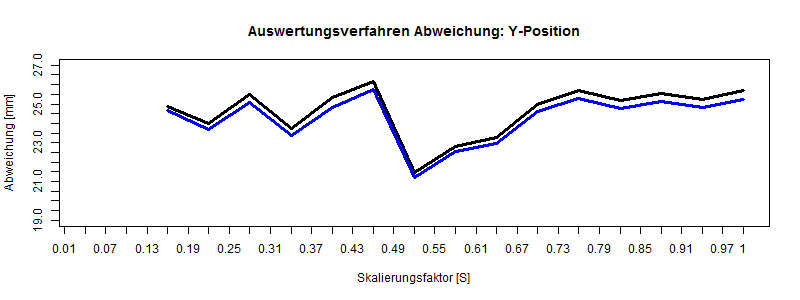
\includegraphics[width=\linewidth]{img_Skalierung/Verfahren_TY}
	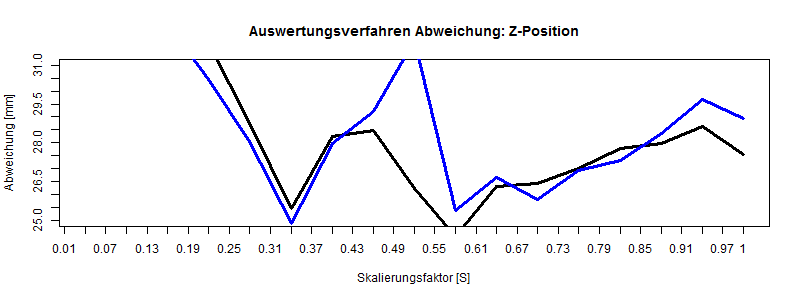
\includegraphics[width=\linewidth]{img_Skalierung/Verfahren_TZ}
	\caption{Dargestellt ist der Median der Abweichung in Millimeter der Positionsbestimmung auf Bilder die mit Lanczos skaliert wurden.\\
	PoseWorld (schwarz), PoseCamera (rot, verdeckt von PW), CorrectPoseCamera (grün, verdeckt von CPW) und CorrectPoseWorld (blau)\\
	Oben: X-Position, Mitte: Y-Position, Unten: Z-Position}
	\label{img_Verfahren_Pos}
\end{figure}
\subsubsection{Orientierung}
Bei der Rotation zeigen sich nun Unterschiede zwischen den einzelnen Verfahren, da bei PoseWorld und CorrectPoseWorld auch die Position im Kamerabild berücksichtigt wird.\\
Aus \autoref{img_Verfahren_Rot} ist zu entnehmen, dass die zusätzliche Korrektur das Ergebnis weiter verbessert wird, wenn die Pixelorientierungen mit beachtet werden.
\begin{figure}
	\centering
	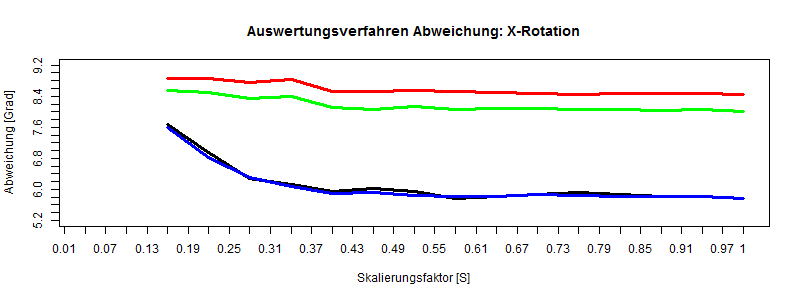
\includegraphics[width=\linewidth]{img_Skalierung/Verfahren_RX}
	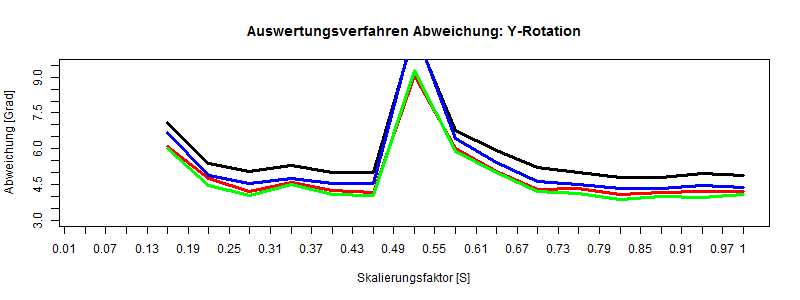
\includegraphics[width=\linewidth]{img_Skalierung/Verfahren_RY}
	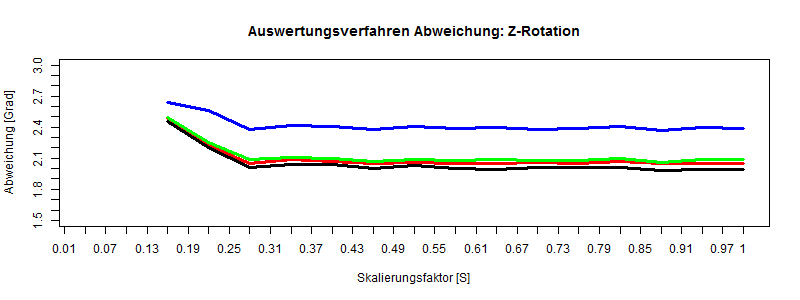
\includegraphics[width=\linewidth]{img_Skalierung/Verfahren_RZ}
	\caption{Dargestellt ist der Median der Abweichung in Grad der Positionsbestimmung auf Bilder die mit Lanczos skaliert wurden.\\
		PoseWorld (schwarz), PoseCamera (rot), CorrectPoseCamera (grün) und CorrectPoseWorld (blau)\\
		Oben: X-Rotation, Mitte: Y-Rotation, Unten: Z-Rotation}
	\label{img_Verfahren_Rot}
\end{figure}
\subsubsection{Ergebnis}
Es zeigt sich, dass CorrectPoseWorld, also die komplexe Bestimmung der Position mittels 2D/3D Landmarks und zusätzlicher Korrektur der Winkel die besten Ergebnisse liefert im Test.\\
Im Test ist die Überführung von 3D zu 2D Landmarks am besten (CorrectPoseCamera und CorrectPoseWorld) kann sich allerdings auch ändern wenn die Kamera Parameter besser abgeschätzt sind, da ohne eine Tiefenaufnahme die korrekte Überführung nur geschätzt werden kann und sich Fehler fortpflanzen können.
\subsection{Ergebnis bezüglich Verwendbarkeit}
Anhand der Detektionsrate abhängig von der Skalierung, siehe \autoref{img_lineareverkleinerung}, kann entnommen werden, das Gesichter unter 50 Pixel Größe nicht mehr sinnvoll erkannt werden können. Somit ergibt sich eine maximale Distanz von etwa $4,5m$ (basierend auf der Actioncam) für eine Analyse.\\
Da die maximale Distanz auf der gearbeitet werden soll jedoch $(8m)$ beträgt, ergibt sich eine Gesichtsgröße von etwa 22 Pixel. Dies entspricht einer Skalierung von $0,28$ für den BIWI-Datensatz. Bei dieser Bildgröße ist in der Standardanwendung ohne Skalierung keine Detektion möglich.\\
Werden die Bildbereiche hingegen hochskaliert, zeigt der Test, das sogar Gesichter mit einer Größe von unter 22 Pixel (Skalierung $0,25$, $8m$) gefunden und analysiert werden können. Dies bedeutet, dass mit diesem Trick auch mit der Hälfte der Bildinformationen noch gearbeitet werden kann, wenn die Eingabe dadurch dem Trainingsdatensatz eher entspricht.\\
Für eine erfolgreiche Analyse sind die Parameter Detektionsrate, Qualität der Rotation und Qualität der Position relevant. Daher wurden die verschiedenen Skalierungsverfahren in diesen Parametern bei unterschiedlichen Größen der Eingabebilder verglichen.\\
Die höchste Detektionsrate bei den Skalierungen erreicht Bicubic, wobei der Unterschied zu Lanczos und Linear so minimal ausfällt, das sie als Gleichwertig in diesem Bereich betrachtet werden kann. Es zeigt sich auch die deutliche Schwäche von Nearest-Neighbor, die Detektionsrate nimmt deutlich früher ab als bei den anderen.\\
Bei der Bestimmung der Rotation kann nur ein geringer Unterschied zwischen den einzelnen Verfahren erkannt werden. Für die X-Rotation hat das Bicubic-Verfahren einen um etwa $2^\circ$ größeren Fehler als die anderen, bei der der Y-Rotation hingegen $0,8^\circ$ genauer ist. Bei der Z-Rotation ist kein klarer Unterschied zu erkennen, somit ist bei diesem Parameter die Wahl des Verfahrens egal.\\
Zur Bestimmung der Position ist das lineare Verfahren am besten geeignet, da es den kleinsten Fehler aufweist, wobei der Unterschied mit $1mm$ sehr gering ausfällt.\\
Der Test mit dem Pixelrauschen soll etwaige Bildfehler simulieren, wie es bei schlechten Kameras der Fall sein kann, was die Auswertung auf kleinen Bildausschnitten erschwert. Somit kann auch gezeigt werden, dass dieser Trick mit der Vergrößerung auch sehr wahrscheinlich in der späteren Anwendung funktionieren wird. In diesem Test erreicht das lineare Verfahren die höchste Detektionsrate, diesmal ist der unterschied zwischen den einzelnen Verfahren deutlich besser erkennbar.\\
Somit erfüllt das lineare Verfahren die Parameter am besten, wobei der Unterschied zwischen den einzelnen recht gering ausfällt und die Wahl des Skalierungsverfahren von anderen Kriterien abhängig gemacht werden kann, wie z.B. von der Rechenzeit.. Dabei kann vom Nearest-Neighbor abgeraten werden wegen dem deutlich früheren Abfall der Detektionsrate.\\
Theoretisch wären sogar Distanzen bis zu $14m$ ($12$Pixel) möglich, basierend auf der hohen Auflösung der Actioncam für eine erfolgreiche Detektion.\\
Der Unterschied bei Skalierung 1 (Originalgröße) zu der Ergebnissen in Paper \cite{OpenFace} kann an der Verwendung des Median anstelle des Durchschnitts als auch an der verwendung von verschiedenen Kameraparametern liegen.